%mypipes
%texmacs ~/for/fortexmacs/master_extract.tm
\documentclass[12pt]{article} % use larger type; default would be 10pt

\usepackage{xeCJK}
\usepackage{enumerate}
\usepackage{geometry}
%%\usepackage[japanese]{babel}
\usepackage{setspace}
\usepackage{amsmath,amssymb,bbm,xypic}
\usepackage[all,cmtip]{xy}
\usepackage{amsmath,amssymb,bbm,float,mystyle}
\usepackage[normalem]{ulem}
\usepackage{caption}
\usepackage{subcaption}
\usepackage{setspace}
\usepackage{comment}
\usepackage{catchfilebetweentags}
\usepackage{multirow}
\usepackage[table]{xcolor}
\includecomment{versiona}
\usepackage{tikz}
\usepackage{bashful}
\usetikzlibrary{patterns}
\usepackage{bbm}

\setCJKmainfont[AutoFakeBold=true]{Hiragino Mincho Pro} %my Mac

%%%%%%%%%% Start TeXmacs macros
\catcode`\<=\active \def<{
\fontencoding{T1}\selectfont\symbol{60}\fontencoding{\encodingdefault}}
\catcode`\>=\active \def>{
\fontencoding{T1}\selectfont\symbol{62}\fontencoding{\encodingdefault}}
\newcommand{\assign}{:=}
\newcommand{\comma}{{,}}
\newcommand{\nin}{\not\in}
\newcommand{\tmop}[1]{\ensuremath{\operatorname{#1}}}
\newcommand{\tmtextit}[1]{{\itshape{#1}}}
\newcommand{\um}{-}

\newtheorem{theorem}{定理}
\newcommand{\sol}{\mathcal{S}\!{\it ol}(\R^{p,q};\lambda,\nu)}
\newcommand{\Hom}{\mbox{\normalfont Hom}}
\newcommand{\Sol}{\mathcal{S}\!{\it ol}}
\newcommand{\Ind}{\mbox{\normalfont Ind}}
\newcommand{\Supp}{\mathcal{S}\!{\it upp}}
\newtheorem{remark}[theorem]{注}
\newtheorem{corollary}[theorem]{系}
\newtheorem{fact}{Fact}
%\newtheorem{definition}{Definition}
\theoremstyle{definition}
\newtheorem{definition}{定義}

\makeatletter
\newtheoremstyle{exampstyle}
  {\topsep} % Space above
  {\topsep} % Space below
  { {\addtolength{\@totalleftmargin}{3.5cm}
     \addtolength{\linewidth}{-3.5cm}
        \parshape 1 3.5em \linewidth}} % Body font
  {-2.5cm} % Indent amount
  {\bfseries} % Theorem head font
  {.} % Punctuation after theorem head
  {.5em} % Space after theorem head
  {} % Theorem head spec (can be left empty, meaning `normal')
\makeatother

\theoremstyle{exampstyle} \newtheorem{examp}[theorem]{Theorem}

\catcode`\<=\active \def<{
\fontencoding{T1}\selectfont\symbol{60}\fontencoding{\encodingdefault}}
\catcode`\>=\active \def>{
\fontencoding{T1}\selectfont\symbol{62}\fontencoding{\encodingdefault}}
\newcommand{\dueto}[1]{\textup{\textbf{(#1) }}}
\newcommand{\tmrsub}[1]{\ensuremath{_{\textrm{#1}}}}
\newcommand{\tmrsup}[1]{\textsuperscript{#1}}
\newcommand{\tmtextbf}[1]{{\bfseries{#1}}}
\newtheorem{proposition}{Proposition}
\newcommand{\Op}{\mbox{\normalfont Op}}
\newcommand{\Res}{\operatorname{Res}\displaylimits}
\newcommand{\OpR}{\mbox{\it R}}
\renewcommand{\Q}{Q_{p,q}}
\newcommand{\IlambdaGprime}{I(\lambda)\kern-0.3em\mid_{G'}}
\newcommand{\SBO}{\Hom_{G'}\left(\IlambdaGprime,J(\nu) \right)}
\renewcommand{\setminus}{-}
%%%%%%%%%% End TeXmacs macros

\setlength{\parskip}{0.4em}
\setlength{\parindent}{2em}

\newcommand{\even}{2\Z}
\newcommand{\odd}{2\Z+1}
\newcommand{\teven}{\mbox{\textrm{: 具数}}}
\newcommand{\todd}{\mbox{\textrm{: 奇数}}}
\newcommand{\tevenText}[1]{\vspace{-3cm}$\begin{array}{l}\nu\teven\\\nu#1\end{array}$}
\newcommand{\toddText}[1]{\vspace{-3cm}$\begin{array}{l}\nu\todd\\\nu#1\end{array}$}
\newcommand{\bb}{\backslash\backslash}
\renewcommand{\ss}{//}
%%%%%%%%%% End TeXmacs macros

\begin{document}
\renewcommand{\abstractname}{概要}

\title{不定値直交群$O(p,q)$の対称性破れ作用素}

  %%%% 講演者1
\author{小林 俊行\thanks{Partially supported by Grant-in-Aid for Scientific
	Research (A) (25247006), Japan Society for the Promotion of Science.} (東京大学、カブリ数物連携宇宙研究機構)\\
  レオンチエフ アレックス (東京大学)}

  %%%% 講演者2

  %%%% 日付
%  \date{2012年3月26日}

  %%%% 謝辞、キーワード、MSCコード  

  \maketitle
\begin{abstract}
	ペア$(G, G') =(O(p+1, q+1), O(p,q+1))$に対して、$G$の球退化主系列表現から、$G'$の球退化主系列表現への
	全て対称性破れ作用素を構成し、分類する。$q=0$の特別な場合が小林俊行氏とB. Speh氏によって[Memoirs of Amer. Math. Soc. 2015]
	解決された。
	函数等式、留数公式と対称性破れ作用素の像も具体的に述べる。
	この結果は小林氏に提唱された分岐則問題を深く研究するためABCプログラム[Progr. Math. 2015]のCの特別な場合になる。
\end{abstract}

  \begin{versiona}
	  $\R^n$ ($n:=p+q$)上の符号$(p,q)$をもつ標準二次形式を$\Q$と表し、
	  \begin{equation*}
  \Q (x) \assign \,^t \! x I_{p, q} x, \; (x \in
  \mathbbm{R}^{p + q}),
	  \end{equation*}
	  ここで、
\begin{equation*}
   I_{p, q} \assign \tmop{diag} (\underbrace{1, \ldots, 1}_p, \underbrace{-
  1, \ldots, - 1}_q).
\end{equation*}
$G$を$G \assign O (p +
1, q + 1)=\left\{ g\in GL\left( p+q+2,\R \right):\;^t\!gI_{p+1,q+1}g=I_{p+1,q+1} \right\}$とすると、
極大放物型部分群
$P=MAN_{+}$をとる.ここで、
\ExecuteMetaData[.master_extract.tex]{tagsetting}
複素数パラメータ
$\lambda\in\C$に依存する$G$の退化主系列表現を定める
\begin{align*}
I(\lambda)&:=\Ind_P^G(\C_\lambda)\\
&\simeq \left\{ f\in C^{\infty}(G)\mid f(gma(t)n)=e^{-\lambda t}f(g),\;\forall(g,ma(t)n)\in G\times P \right\}.
\end{align*}

$G$の簡約部分群として第$p$座標の固定部分群を$G':=G_{e_{p+1}}:=\mysetn{g \in G}{g \cdot e_{p + 1} = e_{p + 1}}$とする。
そうすると、$G$は$P$と適合する(つまり、$A\subset G'$のため、$P':=P\cap G'$は$G'$のラングランズ分解$P'=(G'\cap M)A(G'\cap N_+)$を持つ極大放物型部分群である)
同じいように、複素数パラメータ$\nu\in\C$に依存する$G'$の退化主系列表現$J(\nu):=\Ind_{P'}^{G'}(\C_{\nu})$を定める。

その設定の上で、本研究は主に$G$-表現$I(\lambda)$から、$G'$-表現$J(\nu)$への$G'$-intertwining作用素(つまり、対称性破れ作用素、或いはSBO)に関する。
対称性破れ作用素の空間を$\SBO$として表す。

\cite{kobayashi2013finite,kobayashi2014classification}の一般論における以下のようなアプリオリ評価がある:
\begin{fact}
	対称性破れ作用素空間の次元が表現のパラーメタ$(\lambda,\nu)$よらずに一様に押さえられている。
\end{fact}
以下の定理\ref{thm:classif}で、$\SBO$空間の規定を具体的に述べる。

$\SBO$を理解するため、まず以下のような定義する:
\begin{definition} \label{def1}
	$h(b,x):=1-2\,^t\!bI_{p,q}x+\Q(b)\Q(x)$とする (ここで、$b,x\in\R^{n}\;(n=p+q)$). 超関数
	$F \in \mathcal{D}' (\R^{p,q})$は、
	全て$b_p=0$を満たす$b\in\R^n$と開集合$\mysetn{x\in\R^{p,q}}{h(b,x)\neq0}$に入っている$x$に対して、
  \begin{equation*}
    \label{eq-Nequiv} | h(b,x) |^{\lambda - n} F \left(
    \frac{x - \Q (x) b}{h(b,x)} \right) = F (x)\mbox{ が成り立つと、}
  \end{equation*}
  \tmtextit{$N_+'$不変}と呼ばれる。
\end{definition}

%%	そうすると、$G$は$P$と適合する(つまり、$A\subset G'$のため、$P':=P\cap G'$は$G'$のラングランズ分解$P'=(G'\cap M)A(G'\cap N_+)$を持つ極大放物型部分群である)
%%	同じいように、複素数パラメータ$\nu\in\C$に依存する$G'$の退化主系列表現$J(\nu):=\Ind_{P'}^{G'}(\C_{\nu})$を定める。
%%	$G$の簡約部分群として第$p$座標の固定部分群を$G':=G_{e_{p+1}}:=\mysetn{g \in G}{g \cdot e_{p + 1} = e_{p + 1}}$とする。
\begin{definition}\label{def2}
	$O(p-1,q)$を$\R^n$ $(n=p+q)$に$p$座標を固定するような作用を考える。
	以下のような条件を満たす超関数$F\in\mathcal{D}'(\R^n)$空間を$\sol$として表せる:
\begin{enumerate}[(1)]
    \item $F (x) = F (- x)$;
    \item $F$は$O(p-1,q)$不変である;
    \item $F$は$\lambda-\nu-n$-次の斉次性を持つ;
    \item $F$は$\R^{p,q}$上に$N_+'$不変である;
  \end{enumerate}
\end{definition}
\end{versiona}

\cite[Chap.\ 3]{kobayashi2015symmetry}で証明された一般理論を今の特別な設定に適
用すると、以下のFact\footnote{is there any good translation of ``fact'' to japanese?}式を得ます。
\begin{fact}[{\cite[Thm. 3.16]{kobayashi2015symmetry}}]\label{fact1}
$n:=p+q$とする。
以下の図式が可換である:
\begin{figure}[H]
\centerline{
	\xymatrixcolsep{5pc}
	\xymatrix{\SBO\ar[r]^{\simeq} \ar@/^2pc/[rr]^{\Supp}
	&\left( \mathcal{D}'(G/P,\mathcal{L}_{n-\lambda}) \otimes\mathbb{C}_\nu \right)^{P'}
\ar[r]_-{F\mapsto \supp(F)}\ar[d]^{\simeq}_{\mbox{rest}}
&2^{P'\backslash G/P}\\
&{\hspace{1.65cm}\sol\subset\mathcal{D}'(\R^{p,q})}\ar[lu]^{\mbox{Op}}_{\simeq}&
}
}
\end{figure}
\end{fact}

特に、$T\in\SBO$に対して, $\Supp(T)$は$P'\backslash G/P$の閉部分集合である。
なので、有限両側剰余空間$P'\backslash G/P$の
閉部分集合が対称性破れ作用素の大切な
invariantになるということがわかる。
従って、対称性破れ作用素を分類するため、最初のステップとして、両側剰余空間$P'\backslash G/P$とその閉包関係を決定する。

$G=O(p+1,q+1)$の$\R^{p+1,q+1}$にの自然作用は
$\Xi^{p+1,q+1}:=\mysetn{(x,y)\in\R^{p+1,q+1}\setminus\left\{ 0 \right\}}{\myabs{x}^2=\myabs{y}^2}$を不変にするので\footnote{I am not sure in this japanese},
商空間
$X^{p,q}:=\Xi^{p+1,q+1}/\R^{\times}$にも自然に作用する。
幾何的に、$X^{p,q}$は
$G$は共形変換群として作用する
不定値計量$g_{\Sp^p}\oplus \left( -g_{\Sp^q} \right)$を持つ
関多様体直積多様体$\Sp^p\times\Sp^q$から
対跡点を同ー視することによって得られる商多様体
と同値である。

\[
	X:=G/P\simeq X^{p,q},\quad Y:=\mysetn{[\xi:\eta]\in G/P\simeq X^{p,q}}{\xi_{p}=0}\simeq X^{p-1,q}\]
	\[C:=\mysetn{[\xi:\eta]\in G/P\simeq X^{p,q}}{\xi_{0}=\eta_q}\simeq X^{p-1,q-1}\cup\Xi^{p,q},\quad\left\{ [o] \right\}:=\left\{ [1:0_{p+q}:1] \right\}\mbox{とする.}\]
\begin{theorem}[$G/P$の$P'$不変閉部分集合の分類]
	$p,q\ge1$とする。
	$G/P$の$P'$不変閉部分集合が以下のHasse図式で記述される。ここで
	$
	\begin{array}{l}
	        \xymatrixrowsep{0.5pc}
		\xymatrix{A\ar@{-}[d]^m\\B}
	\end{array}
	$
	は$A\supset B$と$B$のジェネリック部分が$A$の中余次元$m$を持つということが表している。\\
  \begin{figure}[H]
    \centering
    \begin{subfigure}[t]{0.3\textwidth}
	    \xymatrixrowsep{0.5pc}
	    \xymatrix{&X\ar@{-}[ld]_1\ar@{-}[rd]^1&\\Y\ar@{-}[rd]_1&&C\ar@{-}[ld]^1\\&C\cap Y\ar@{-}[dd]^{p+q-2}&\\&&\\&\{[o]\}&}
	\caption{$p>1$のとき}
    \end{subfigure}
    ~ %add desired spacing between images, e. g. ~, \quad, \qquad, \hfill etc. 
      %(or a blank line to force the subfigure onto a new line)
    \begin{subfigure}[t]{0.3\textwidth}
	    \xymatrixrowsep{0.5pc}
	    {\xymatrix{&X\ar@{-}[ld]_1\ar@{-}[rd]^1&\\Y\ar@{-}[rddd]_{p+q-2}&&C\ar@{-}[lddd]^{p+q-2}\\&&\\&&\\&\{[o]\}&}}
	\caption{$p=1$のとき}
    \end{subfigure}
\end{figure}
\end{theorem}
$P'\backslash G/P$のそれぞれの閉集合$S$に対して、対称性破れ作用素のファミーリ$R^S_{\lambda,\nu}$を構成する。更に、
\begin{itemize}
	\item $R_{\lambda,\nu}^S$は$(\lambda,\nu)\in D_S$に対して定義されている。ここで、$D_S$は$\C^2$の部分集合である(もっと詳しくいうと、
		$\C^2$全体或いは1次元アフィン空間の加算和である);
	\item $R_{\lambda,\nu}^S$は$(\lambda,\nu)\in D_S$に正則に依存する;
	\item 全て$(\lambda,\nu)\in D_S$に対して、$\Supp(R_{\lambda,\nu}^S)\subset S$である(更に、ジェネリック$(\lambda,\nu)$的に、等式が成り立つ).
\end{itemize}
この作用素はある点でゼロになることがあり得る(注意\ref{rmk:thm:construction}のよう)。
従って、$\tilde{R}^X_{\lambda,\nu}$という対称性破れ作用素のファミリを再規準化として定義する。
しかし、$p=1$のとき、$S=C-cap Y$の場合と$p>1$のとき、$S=C$又は$Y$の場合は以下に出てくる分類(定理\ref{thm:classif})に出てこないので、
省略する。
\newpage
\begin{theorem}[対称性破れ作用素の構成]\label{thm:construction}
	$S=X,Y,C,$と$\left\{ o \right\}$に対して、以下の$R_{\lambda,\nu}^S$と$\tilde{R}_{\lambda,\nu}^X$作用素は$(\lambda,\nu)\in D_S$に正則に依存する
	$\IlambdaGprime$から$J(\nu)$への対称性破れ作用素である。\\
\ExecuteMetaData[.master_extract.tex]{table}\vspace{\baselineskip}
表の記号を説明する:
\begin{itemize}
	\item $\mid \mid \mid \assign \{ (\lambda, \nu) \in \mathbbm{C}^2 \mid \nu \in
	- 2\mathbbm{N} \cup (q + 1 + 2\mathbbm{Z}) \},\quad \backslash\backslash:=\mysetn{(\lambda,\nu)\in\C^2}{\lambda+\nu-n+1\in-2\N}$;
\item $/ / \assign
\{ (\lambda, \nu) \in \mathbbm{C}^2 \mid \lambda - \nu \in
-2\N \},\quad \mid\mid:=\mysetn{(\lambda,\nu)\in\C^2}{\nu\in1+2\N}$;
\item $\tilde{C}(s,t)$は\cite[(16.3)]{kobayashi2015symmetry}のように定義される、
	renormalized Gegenbauer多項式から導入される2変数多項式である。
\end{itemize}
\end{theorem}
$(\lambda,\nu)\in\mid\mid$に対して、$m:=\frac{1}{2}\left( \nu-1 \right)\in\N$とし、$(\lambda,\nu)\in\bb$に対して、$k:=\frac{1}{2}\left( n-1-\lambda-\nu \right)\in\N$とする。
$p=1$に対して、$q_C^X(\lambda,\nu)$ and $q_Y^X(\lambda,\nu)$を以下のように定義する:
\ExecuteMetaData[.master_extract.tex]{residue}
\begin{remark}
	\cite[Chap.\ 2]{kobayashi2016differential1}の微分対称性破れ作用素の一般論によって、
	$S=\left\{ o \right\}$ならば、$R_{\lambda,\nu}^S$は微分作用素である。
	定義によって、定理\ref{thm:construction}の$R_{\lambda,\nu}^{ \left\{ o \right\}}$を以下のように述べる:
	\begin{equation*}
		R_{\lambda,\nu}^{ \left\{ o \right\}}=
		\sum_{j=0}^{\frac{\nu-\lambda}{2}}\frac{(-1)^j2^{\nu-\lambda-2j}}{j!(\nu-\lambda-2j)!}\prod_{i=1}^{\frac{\nu-\lambda}{2}-j}\left( \frac{n
		+1}{2}+\frac{\nu+\lambda}{2}
		+i \right)\left(- \Delta_{\mathbbm{R}^{p-1,q}} \right)^j\left( \frac{\partial}{\partial x_p} \right)^{\nu-\lambda-2j}.
	\end{equation*}
	上の公式の$q=0$の特別な場合が\cite[Thms. 5.1.1 and 5.2.1]{juhl2009families}と\cite[(10.1)]{kobayashi2015symmetry}に出てきて、
	一般の$p,q$の場合は
	\cite[Thm.\ 4.3]{kobayashi2015branching}に出てきた。
\end{remark}
\begin{remark}\label{rmk:thm:construction}
	定理\ref{thm:construction}の表の一番右の列からわかるのは、全ての$(\lambda,\nu)\in\C^2$に$R_{\lambda,\nu}^{ \left\{ o \right\}},R_{\lambda,\nu}^Y,R_{\lambda,\nu}^C\neq0$、
	$R^X_{\lambda,\nu}=0\iff(\lambda,\nu)$が以下の離散集合に入っている:
	\[\begin{cases}
			//\cap\mid\mid\mid,&p>1,\\
			\mybra{//\cap\mid\mid\mid} \cup \mybra{\backslash\backslash\cap\mid\mid},&p=1,
		\end{cases}
	\]
	and $\tilde{R}_{\lambda,\nu}^X=0\iff p=1$、$(\lambda,\nu)$は離散集合$\backslash\backslash\cap \mid\mid$に入っている.
\end{remark}
定理\ref{thm:construction}で構成される対称性破れ作用素はいつも線型独立になるとは限らないが、全ての対称性破れ作用素を生成する。
全ての$(\lambda,\nu)\in\C^2$に対して、$\SBO$の基底を以下のように具体的に述べる:
\begin{theorem}[対称性破れ作用素の分類]\label{thm:classif}
	$p,q\ge1$とする.
		\ExecuteMetaData[.master_extract.tex]{classification}
\end{theorem}
\begin{corollary}\label{cor:classif}
	$(\lambda,\nu)\in\C^2$に、
	$\dim_{\C}\SBO\in\left\{ 1,2 \right\}$が成り立つ。
\end{corollary}
$G$の球退化主系列表現$I(\lambda)$は球ベクトル(或いは、$K$不変ベクトル)の1次元部分空間を持つ。$G'$表現$J(\nu)$も同じようである。
$\mathbbm{1}_\lambda\in I(\lambda)^K,\mathbbm{1}_\nu\in J(\nu)^{K'}$を$\mathbbm{1}_\lambda(e)=\mathbbm{1}_\nu(e)=1$
のように正則化された球ベクトルとする。そのように正則化をすると、以下のことが成り立つ:
\begin{theorem}[球ベクトルのスペクトラム]\label{thm:spherical}
	前のように、$n:=p+q\;(p,q\ge1)$とする。そうすると、
\[ \OpR^X_{\lambda, \nu} \mathbbm{1}_{\lambda} =  \frac{2^{1 -
\lambda}\pi^{n / 2}}{\Gamma \left( \frac{\lambda}{2} \right)
\Gamma \left(  \frac{\lambda + 1-q}{2} \right) \Gamma \left(
\frac{q - \nu + 1}{2} \right)} \mathbbm{1}_{\nu}\mbox{ が成り立つ。}\]
\end{theorem}
\begin{remark}
	定理\ref{thm:spherical}の$p=q=1$の特別な場合が\cite[Lem. A.5]{bernstein2004estimates} に知られている。
	これの高階設定に一般化が\cite[Thm. 1.1]{clerc2011generalized}である。
	$q=0$の場合が\cite[Prop.\ 7.4]{kobayashi2015symmetry}に述べられている。
\end{remark}
$(\lambda,\nu)\in\C^2\setminus//$に対して、
\[K_{\lambda,\nu}^{\mathbb{R}^{p,q}}:=\frac{\myabs{x_p}^{\lambda+\nu-n}}{\Gamma\left( \frac{\lambda+\nu-n+1}{2} \right)}\times
\frac{\myabs{\Q}^{-\nu}}{\Gamma\left( \frac{1-\nu}{2} \right)}\in\sol\mbox{を定義する。}\]
そうすると、$R_{\lambda,\nu}^X=\frac{1}{\Gamma\left( \frac{\lambda-\nu}{2} \right)}\Op\left( K_{\lambda,\nu}^X \right)$.
これの左辺は$(\lambda,\nu)\in\C^2$に正則に依存する対称性破れ作用素のファミリに拡張できる。
\begin{theorem}[留数公式]
	前のように、$n:=p+q\;(p,q\ge1)$とする。
	$(\lambda,\nu)\in//$に対して、$l:=\frac{1}{2}\left( \nu-\lambda \right)\in\N$とする。そうすると、
  \[\OpR_{\lambda,\nu}^X  = \frac{ (- 1)^l l!\pi^{(n - 2) / 2} 
		}{2^{ \nu + 2 l-1}}\cdot  \frac{\sin\left( \frac{1+q-\nu}{2}\pi \right)}{\Gamma\left( \frac{\nu}{2} \right)}
     \OpR_{\lambda,\nu}^{ \left\{ o \right\} },\quad(\lambda,\nu)\in// . \]
	\end{theorem}
	\begin{remark}
		留数公式の$q=0$の場合は\cite[Thm. 12.2]{kobayashi2015symmetry}に示された。
	\end{remark}
	\begin{definition}
		\ref{fact1}の建設のように、$G=O(p+1,q+1)$に$\Hom_G(I(\lambda),I(\nu))\simeq\Sol_G(\R^{p,q};\lambda,\nu)$である。
		ここで、$\Sol_G(\R^{p,q};\lambda,\nu)\subset\mathcal{D}'(\R^{p+q})$は定義\ref{def2}の4つ科目を満たす$\R^{p+q}$上の超関数空間(しかし、
		3つ目の科目で$O(p,q)_{e_p}$不変性の代わりに、$O(p,q)$を求め、
		4つ目の科目で$N_+'$不変性の代わりに、$N_+$不変性を求める;$N_+$不変性の定義が$N_+'$不変性と全く同じが、定義で$b_p$をもとめられない)。

		以下のように定義された超関数は
		\begin{equation*}
			\myabs{\Q}^{\lambda-n}\times\begin{cases}
				\Gamma^{-1}\left( \lambda-n/2 \right),&\min\left\{ p,q \right\}=0,\\
				\Gamma^{-1}\left( \frac{\lambda-n+1}{2} \right)\Gamma^{-1}\left( \lambda-n/2 \right),&\min\left\{ p,q \right\}>0,n\in2\Z+1,\\
  \Gamma^{-1} \left( \frac{\lambda-n + 1}{2} \right) \Gamma ^{-1}\left( \frac{\lambda-n/2+
  1}{2} \right), &\min\left\{ p,q \right\}>0, n / 2 + p \in 2\mathbbm{Z}+ 1,\\
  \Gamma^{-1} \left( \frac{\lambda-n + 1}{2} \right) \Gamma ^{-1}\left( \frac{\lambda-n/2}{2}
  \right), & \min\left\{ p,q \right\}>0,n / 2 + p \in 2\mathbbm{Z}
			\end{cases}
		\end{equation*}
		$\Sol_G(\R^{p,q};\lambda,n-\lambda)$に入っている。
		これを積分核として用い、$G=O(p+1,q+1)$intertwining作用素
		$\tilde{\mathbb{T}}^{G}_{\lambda}:I(\lambda)\to
		I(n-\lambda)$
		を定められる
		(\textit{Knapp--Stein 作用素})。
		$G$の代わりに$G'=O(p,q+1)$を代入して、に対して全く同じように建設すれば、$\tilde{\mathbb{T}}^{G'}_\nu:J(\nu)\to J(n-1-\nu)$作用素をえる。
	\end{definition}
	\begin{theorem}[函数等式]
	前のように、$n:=p+q\;(p,q\ge1)$とする。
	そうすると、
\ExecuteMetaData[.master_extract.tex]{functional}
	\end{theorem}
	\begin{remark}
		函数等式の特別の$q=0$の場合は\cite[Thm. 12.6]{kobayashi2015program}に示された。
	\end{remark}
	$G'=O(p,q+1)$表現$J(\nu)$ of $G'=O(p,q+1)$は $K'$表現として multiplicity-freeであるので、$p>1$のとき、これの $(\mathfrak{g}',K')$部分加群を $\N_{+}^2$の部分集合で表すことができる。
	ここで$J(\nu)$の$K'$表現の構造は球面調和関数
	$\mathcal{H}^a(\Sp^{p-1})\boxtimes\mathcal{H}^b(\Sp^q)$で表せる。
 	\cite{howe1993homogeneous}のように、$J(\nu)$のJordan--H\"older 列 (或いは、socle filtrations) を矢印で表す。
	そうすると:
\begin{theorem}[対称性破れ作用素の像]
	The regular SBO $R_{\lambda,\nu}^X:I(\lambda)\to J(\nu)$ is surjective,
	$\nu\in\Z$ではなかったら、regular対称性破れ作用素$R_{\lambda,\nu}^X:I(\lambda)\to J(\nu)$は射影関数である。
	$\nu\in\Z$ならば、$(\mathfrak{g},K)$加群 $I(\lambda)_K$の
	$R_{\lambda,\nu}^X$における像は以下のようになる(ここで$(\lambda,\nu)\in//$に対して、
	$l:=\frac{1}{2}\left( \nu-\lambda \right)\in\N$、$(\lambda,\nu)\in\backslash\backslash$に対して、$k:=\frac{1}{2}\left( n-1-\lambda-\nu \right)
	\in\N$ である; 障壁 $A^{\pm\pm}$
	が\cite{howe1993homogeneous}のように定義する): \\
	for $p>1$:
\end{theorem}
\begin{enumerate}[(1)]
	\item $p\in2\N_++1$ と $q\in2\Z$とする. そうすると、$\nu\in2\Z,0<\nu<n-1$ならば、$R_{\lambda,\nu}^X$ は射影函数である。そうではなかったら、
		\hspace*{-1cm}\begin{figure}[H]
			\noindent\begin{tabular}{m{1.3cm}rrr}
	      $(\lambda,\nu)\in$&$\mybra{//\cup\backslash\backslash}^c$ & $\backslash\backslash-//$  & $//\cap\backslash\backslash,k> l$\\[0pt]
	      {\vspace{-3cm} $ \begin{array}{l}
	      \nu\teven\\ \nu\le0
      \end{array}$}&{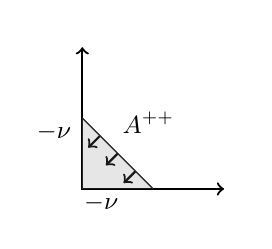
\begin{tikzpicture}[scale=0.6]
\draw [<->,thick] (0.0,3.0) node (yaxis) [above] {}
	|- (3.0,0.0) node (xaxis) [right] {};
\draw (0,1.5)  -- (1.5,0) ;
\draw [thick,->] (0.375,1.125) -- (0.125,0.875);
\draw [thick,->] (0.75,0.75) -- (0.5,0.5);
\draw [thick,->] (1.125,0.375) -- (0.875,0.125);
\node at (1.4,1.4) {\small $A^{++}$};
\node at (0.3999999999999999,-0.3) {\small $-\nu$};
\node at (-0.6,1.2) {\small $-\nu$};
\draw [fill=gray,opacity=0.2,gray] (1.5,0.0) -- (0.0,1.5) -- (0.0,0.0) ;
\end{tikzpicture}}\kern0.7cm
&{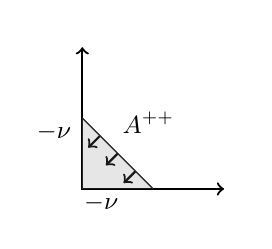
\begin{tikzpicture}[scale=0.6]
\draw [<->,thick] (0.0,3.0) node (yaxis) [above] {}
	|- (3.0,0.0) node (xaxis) [right] {};
\draw (0,1.5)  -- (1.5,0) ;
\draw [thick,->] (0.375,1.125) -- (0.125,0.875);
\draw [thick,->] (0.75,0.75) -- (0.5,0.5);
\draw [thick,->] (1.125,0.375) -- (0.875,0.125);
\node at (1.4,1.4) {\small $A^{++}$};
\node at (0.3999999999999999,-0.3) {\small $-\nu$};
\node at (-0.6,1.2) {\small $-\nu$};
\draw [fill=gray,opacity=0.2,gray] (1.5,0.0) -- (0.0,1.5) -- (0.0,0.0) ;
\end{tikzpicture}}\kern0.7cm
&{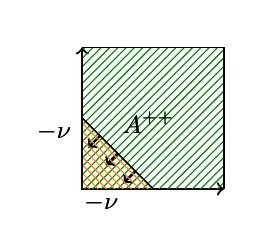
\begin{tikzpicture}[scale=0.6]
\draw [<->,thick] (0.0,3.0) node (yaxis) [above] {}
	|- (3.0,0.0) node (xaxis) [right] {};
\draw (0,1.5)  -- (1.5,0) ;
\draw [thick,->] (0.375,1.125) -- (0.125,0.875);
\draw [thick,->] (0.75,0.75) -- (0.5,0.5);
\draw [thick,->] (1.125,0.375) -- (0.875,0.125);
\node at (1.4,1.4) {\small $A^{++}$};
\node at (0.3999999999999999,-0.3) {\small $-\nu$};
\node at (-0.6,1.2) {\small $-\nu$};
\draw [pattern=north east lines, pattern color=green!50!black] (3.0,0.0) -- (3.0,3.0) -- (0.0,3.0) -- (0.0,0.0) ;
\draw (0,1.5)  -- (1.5,0) ;
\draw [thick,->] (0.375,1.125) -- (0.125,0.875);
\draw [thick,->] (0.75,0.75) -- (0.5,0.5);
\draw [thick,->] (1.125,0.375) -- (0.875,0.125);
\node at (1.4,1.4) {\small $A^{++}$};
\node at (0.3999999999999999,-0.3) {\small $-\nu$};
\node at (-0.6,1.2) {\small $-\nu$};
\draw [pattern=north west lines, pattern color=orange] (1.5,0.0) -- (0.0,1.5) -- (0.0,0.0) ;
\end{tikzpicture}}\kern0.7cm
\\[0pt]
      \vspace{-3cm}$\begin{array}{l}
	      \nu\todd\\ \nu\le\frac{n-3}{2}
      \end{array}$&\input{f2}\\[0pt]
	      $(\lambda,\nu)\in$&$\mybra{//\cup\backslash\backslash}^c$ && $//\cap\backslash\backslash,k=l$\\[0pt]
	      \vspace{-3cm}$\begin{array}{l}\nu\todd\\\nu=\frac{n-1}{2}
	      \end{array}$&\input{f3}\\[0pt]
	      $(\lambda,\nu)\in$&$\mybra{//\cup\backslash\backslash}^c$ & $//-\backslash\backslash$  & $//\cap\backslash\backslash,k< l$\\[0pt]
	      \vspace{-3cm}$\begin{array}{l}\nu\teven\\\nu\ge{n-1}\end{array}$&{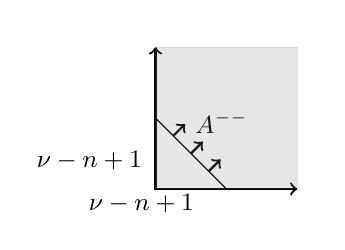
\begin{tikzpicture}[scale=0.6]
\draw [<->,thick] (0.0,3.0) node (yaxis) [above] {}
	|- (3.0,0.0) node (xaxis) [right] {};
\draw (0,1.5)  -- (1.5,0) ;
\draw [thick,->] (0.375,1.125) -- (0.625,1.375);
\draw [thick,->] (0.75,0.75) -- (1.0,1.0);
\draw [thick,->] (1.125,0.375) -- (1.375,0.625);
\node at (-1.4,0.6) {\small $\nu-n+1$};
\node at (-0.30000000000000004,-0.3) {\small $\nu-n+1$};
\node at (1.4,1.4) {\small $A^{--}$};
\draw [fill=gray,opacity=0.2,gray] (3.0,0.0) -- (3.0,3.0) -- (0.0,3.0) -- (0.0,0.0) ;
\end{tikzpicture}}\kern0.7cm
&{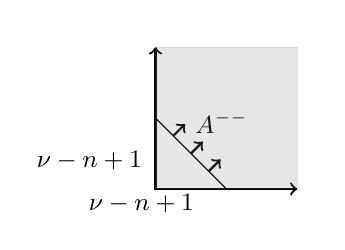
\begin{tikzpicture}[scale=0.6]
\draw [<->,thick] (0.0,3.0) node (yaxis) [above] {}
	|- (3.0,0.0) node (xaxis) [right] {};
\draw (0,1.5)  -- (1.5,0) ;
\draw [thick,->] (0.375,1.125) -- (0.625,1.375);
\draw [thick,->] (0.75,0.75) -- (1.0,1.0);
\draw [thick,->] (1.125,0.375) -- (1.375,0.625);
\node at (-1.4,0.6) {\small $\nu-n+1$};
\node at (-0.30000000000000004,-0.3) {\small $\nu-n+1$};
\node at (1.4,1.4) {\small $A^{--}$};
\draw [fill=gray,opacity=0.2,gray] (3.0,0.0) -- (3.0,3.0) -- (0.0,3.0) -- (0.0,0.0) ;
\end{tikzpicture}}\kern0.7cm
&{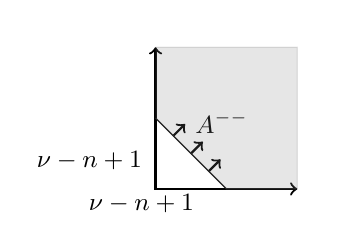
\begin{tikzpicture}[scale=0.6]
\draw [<->,thick] (0.0,3.0) node (yaxis) [above] {}
	|- (3.0,0.0) node (xaxis) [right] {};
\draw (0,1.5)  -- (1.5,0) ;
\draw [thick,->] (0.375,1.125) -- (0.625,1.375);
\draw [thick,->] (0.75,0.75) -- (1.0,1.0);
\draw [thick,->] (1.125,0.375) -- (1.375,0.625);
\node at (-1.4,0.6) {\small $\nu-n+1$};
\node at (-0.30000000000000004,-0.3) {\small $\nu-n+1$};
\node at (1.4,1.4) {\small $A^{--}$};
\draw [fill=gray,opacity=0.2,gray] (0.0,1.5) -- (1.5,0.0) -- (3.0,0.0) -- (3.0,3.0) -- (0.0,3.0) ;
\end{tikzpicture}}\kern0.7cm
\\[0pt]
	    \end{tabular}
	  \end{figure}
		\begin{figure}[H]
			\noindent\begin{tabular}{m{1.3cm}rrr}
	      $(\lambda,\nu)\in$&$\mybra{//\cup\backslash\backslash}^c$ & $//-\backslash\backslash$  & $//\cap\backslash\backslash,k< l$\\[0pt]
	      \vspace{-3cm}$\begin{array}{l}\nu\todd\\\nu\ge\frac{n+1}{2}\end{array}$&\input{f5}\\[25pt]
	    \end{tabular}
	  \end{figure}
	\item $p,q\in\odd$と $p>1$とする。そうすると、
		\begin{figure}[H]
			\noindent\begin{tabular}{m{1.3cm}rrr}
			$(\lambda,\nu)\in$&$\mybra{\ss\cup\bb}^c$ & $\bb-\ss$  & $\ss-\bb$\\[0pt]
			\tevenText{\le0}&{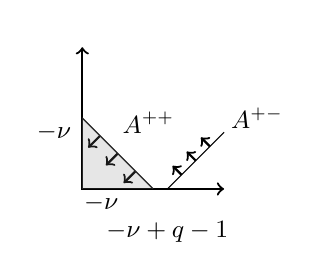
\begin{tikzpicture}[scale=0.6]
\draw [<->,thick] (0.0,3.0) node (yaxis) [above] {}
	|- (3.0,0.0) node (xaxis) [right] {};
\draw (0,1.5)  -- (1.5,0) ;
\draw [thick,->] (0.375,1.125) -- (0.125,0.875);
\draw [thick,->] (0.75,0.75) -- (0.5,0.5);
\draw [thick,->] (1.125,0.375) -- (0.875,0.125);
\node at (1.4,1.4) {\small $A^{++}$};
\node at (0.3999999999999999,-0.3) {\small $-\nu$};
\node at (-0.6,1.2) {\small $-\nu$};
\draw [fill=gray,opacity=0.2,gray] (1.5,0.0) -- (0.0,1.5) -- (0.0,0.0) ;
\draw (1.8,0.0) -- (3.0,1.2) ;
\draw [thick,->] (2.1,0.3) -- (1.9100000000000001,0.49);
\draw [thick,->] (2.4,0.6) -- (2.21,0.79);
\draw [thick,->] (2.7,0.8999999999999999) -- (2.5100000000000002,1.0899999999999999);
\node at (3.7,1.5) {\small $A^{+-}$};
\node at (1.8,-0.9) {\small $-\nu+q-1$};
\end{tikzpicture}\kern-0.7cm}
&{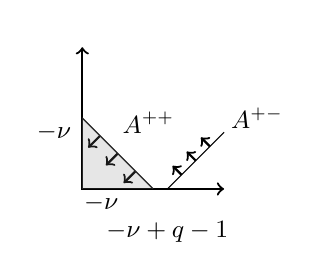
\begin{tikzpicture}[scale=0.6]
\draw [<->,thick] (0.0,3.0) node (yaxis) [above] {}
	|- (3.0,0.0) node (xaxis) [right] {};
\draw (0,1.5)  -- (1.5,0) ;
\draw [thick,->] (0.375,1.125) -- (0.125,0.875);
\draw [thick,->] (0.75,0.75) -- (0.5,0.5);
\draw [thick,->] (1.125,0.375) -- (0.875,0.125);
\node at (1.4,1.4) {\small $A^{++}$};
\node at (0.3999999999999999,-0.3) {\small $-\nu$};
\node at (-0.6,1.2) {\small $-\nu$};
\draw [fill=gray,opacity=0.2,gray] (1.5,0.0) -- (0.0,1.5) -- (0.0,0.0) ;
\draw (1.8,0.0) -- (3.0,1.2) ;
\draw [thick,->] (2.1,0.3) -- (1.9100000000000001,0.49);
\draw [thick,->] (2.4,0.6) -- (2.21,0.79);
\draw [thick,->] (2.7,0.8999999999999999) -- (2.5100000000000002,1.0899999999999999);
\node at (3.7,1.5) {\small $A^{+-}$};
\node at (1.8,-0.9) {\small $-\nu+q-1$};
\end{tikzpicture}\kern-0.7cm}
&{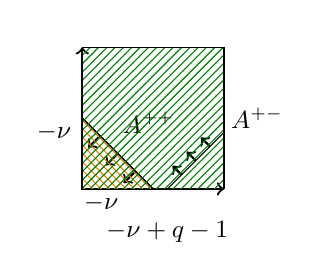
\begin{tikzpicture}[scale=0.6]
\draw [<->,thick] (0.0,3.0) node (yaxis) [above] {}
	|- (3.0,0.0) node (xaxis) [right] {};
\draw (0,1.5)  -- (1.5,0) ;
\draw [thick,->] (0.375,1.125) -- (0.125,0.875);
\draw [thick,->] (0.75,0.75) -- (0.5,0.5);
\draw [thick,->] (1.125,0.375) -- (0.875,0.125);
\node at (1.4,1.4) {\small $A^{++}$};
\node at (0.3999999999999999,-0.3) {\small $-\nu$};
\node at (-0.6,1.2) {\small $-\nu$};
\draw [pattern=north west lines, pattern color=orange] (1.5,0.0) -- (0.0,1.5) -- (0.0,0.0) ;
\draw (1.8,0.0) -- (3.0,1.2) ;
\draw [thick,->] (2.1,0.3) -- (1.9100000000000001,0.49);
\draw [thick,->] (2.4,0.6) -- (2.21,0.79);
\draw [thick,->] (2.7,0.8999999999999999) -- (2.5100000000000002,1.0899999999999999);
\node at (3.7,1.5) {\small $A^{+-}$};
\node at (1.8,-0.9) {\small $-\nu+q-1$};
\draw [pattern=north east lines, pattern color=green!50!black] (3.0,0.0) -- (3.0,3.0) -- (0.0,3.0) -- (0.0,0.0) ;
\end{tikzpicture}\kern-0.7cm}
\\[0pt]
			\toddText{\le n-3}&\input{f7}\\[0pt]
			\tevenText{>0}&\input{f8}\\[0pt]
			\toddText{>n-3}&{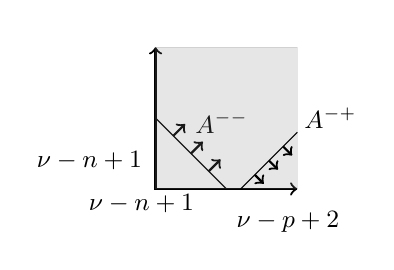
\begin{tikzpicture}[scale=0.6]
\draw [<->,thick] (0.0,3.0) node (yaxis) [above] {}
	|- (3.0,0.0) node (xaxis) [right] {};
\draw (0,1.5)  -- (1.5,0) ;
\draw [thick,->] (0.375,1.125) -- (0.625,1.375);
\draw [thick,->] (0.75,0.75) -- (1.0,1.0);
\draw [thick,->] (1.125,0.375) -- (1.375,0.625);
\node at (-1.4,0.6) {\small $\nu-n+1$};
\node at (-0.30000000000000004,-0.3) {\small $\nu-n+1$};
\node at (1.4,1.4) {\small $A^{--}$};
\draw [fill=gray,opacity=0.2,gray] (3.0,0.0) -- (3.0,3.0) -- (0.0,3.0) -- (0.0,0.0) ;
\draw (1.8,0.0) -- (3.0,1.2) ;
\draw [thick,->] (2.1,0.3) -- (2.29,0.10999999999999999);
\draw [thick,->] (2.4,0.6) -- (2.59,0.41);
\draw [thick,->] (2.7,0.8999999999999999) -- (2.89,0.71);
\node at (3.7,1.5) {\small $A^{-+}$};
\node at (2.8,-0.7) {\small $\nu-p+2$};
\end{tikzpicture}}
&{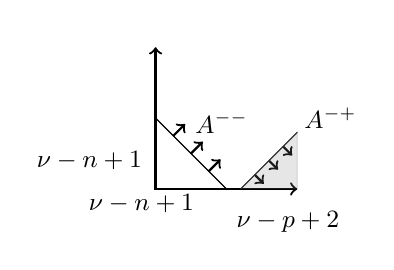
\begin{tikzpicture}[scale=0.6]
\draw [<->,thick] (0.0,3.0) node (yaxis) [above] {}
	|- (3.0,0.0) node (xaxis) [right] {};
\draw (0,1.5)  -- (1.5,0) ;
\draw [thick,->] (0.375,1.125) -- (0.625,1.375);
\draw [thick,->] (0.75,0.75) -- (1.0,1.0);
\draw [thick,->] (1.125,0.375) -- (1.375,0.625);
\node at (-1.4,0.6) {\small $\nu-n+1$};
\node at (-0.30000000000000004,-0.3) {\small $\nu-n+1$};
\node at (1.4,1.4) {\small $A^{--}$};
\draw (1.8,0.0) -- (3.0,1.2) ;
\draw [thick,->] (2.1,0.3) -- (2.29,0.10999999999999999);
\draw [thick,->] (2.4,0.6) -- (2.59,0.41);
\draw [thick,->] (2.7,0.8999999999999999) -- (2.89,0.71);
\node at (3.7,1.5) {\small $A^{-+}$};
\node at (2.8,-0.7) {\small $\nu-p+2$};
\draw [fill=gray,opacity=0.2,gray] (1.8,0.0) -- (3.0,1.2) -- (3.0,0.0) ;
\end{tikzpicture}}
&{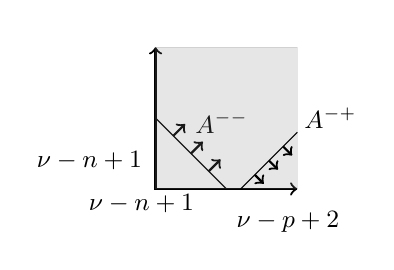
\begin{tikzpicture}[scale=0.6]
\draw [<->,thick] (0.0,3.0) node (yaxis) [above] {}
	|- (3.0,0.0) node (xaxis) [right] {};
\draw (0,1.5)  -- (1.5,0) ;
\draw [thick,->] (0.375,1.125) -- (0.625,1.375);
\draw [thick,->] (0.75,0.75) -- (1.0,1.0);
\draw [thick,->] (1.125,0.375) -- (1.375,0.625);
\node at (-1.4,0.6) {\small $\nu-n+1$};
\node at (-0.30000000000000004,-0.3) {\small $\nu-n+1$};
\node at (1.4,1.4) {\small $A^{--}$};
\draw [fill=gray,opacity=0.2,gray] (3.0,0.0) -- (3.0,3.0) -- (0.0,3.0) -- (0.0,0.0) ;
\draw (1.8,0.0) -- (3.0,1.2) ;
\draw [thick,->] (2.1,0.3) -- (2.29,0.10999999999999999);
\draw [thick,->] (2.4,0.6) -- (2.59,0.41);
\draw [thick,->] (2.7,0.8999999999999999) -- (2.89,0.71);
\node at (3.7,1.5) {\small $A^{-+}$};
\node at (2.8,-0.7) {\small $\nu-p+2$};
\end{tikzpicture}}
\\[0pt]
			  
		\end{tabular}
		\end{figure}
	\item $p,q\in\even$とする。 そうすると、
		\begin{figure}[H]
			\noindent\begin{tabular}{m{1.3cm}rrr}
			$(\lambda,\nu)\in$&$\mybra{\ss\cup\bb}^c$ & $\bb-\ss$  & $\ss-\bb$\\[0pt]
			\tevenText{\le0}&{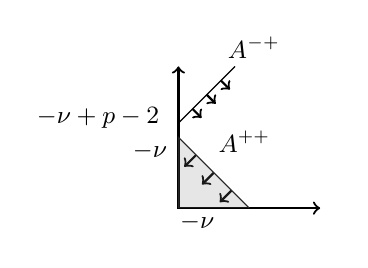
\begin{tikzpicture}[scale=0.6]
\draw [<->,thick] (0.0,3.0) node (yaxis) [above] {}
	|- (3.0,0.0) node (xaxis) [right] {};
\draw (0,1.5)  -- (1.5,0) ;
\draw [thick,->] (0.375,1.125) -- (0.125,0.875);
\draw [thick,->] (0.75,0.75) -- (0.5,0.5);
\draw [thick,->] (1.125,0.375) -- (0.875,0.125);
\node at (1.4,1.4) {\small $A^{++}$};
\node at (0.3999999999999999,-0.3) {\small $-\nu$};
\node at (-0.6,1.2) {\small $-\nu$};
\draw [fill=gray,opacity=0.2,gray] (1.5,0.0) -- (0.0,1.5) -- (0.0,0.0) ;
\draw (0.0,1.8) -- (1.2,3.0) ;
\draw [thick,->] (0.3,2.1) -- (0.49,1.9100000000000001);
\draw [thick,->] (0.6,2.4) -- (0.79,2.21);
\draw [thick,->] (0.8999999999999999,2.7) -- (1.0899999999999999,2.5100000000000002);
\node at (1.6,3.4) {\small $A^{-+}$};
\node at (-1.7,1.9000000000000001) {\small $-\nu+p-2$};
\end{tikzpicture}}
&{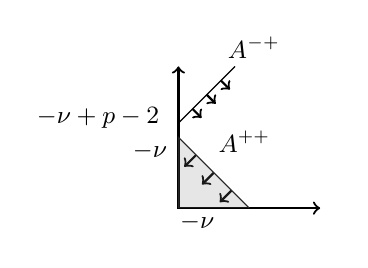
\begin{tikzpicture}[scale=0.6]
\draw [<->,thick] (0.0,3.0) node (yaxis) [above] {}
	|- (3.0,0.0) node (xaxis) [right] {};
\draw (0,1.5)  -- (1.5,0) ;
\draw [thick,->] (0.375,1.125) -- (0.125,0.875);
\draw [thick,->] (0.75,0.75) -- (0.5,0.5);
\draw [thick,->] (1.125,0.375) -- (0.875,0.125);
\node at (1.4,1.4) {\small $A^{++}$};
\node at (0.3999999999999999,-0.3) {\small $-\nu$};
\node at (-0.6,1.2) {\small $-\nu$};
\draw [fill=gray,opacity=0.2,gray] (1.5,0.0) -- (0.0,1.5) -- (0.0,0.0) ;
\draw (0.0,1.8) -- (1.2,3.0) ;
\draw [thick,->] (0.3,2.1) -- (0.49,1.9100000000000001);
\draw [thick,->] (0.6,2.4) -- (0.79,2.21);
\draw [thick,->] (0.8999999999999999,2.7) -- (1.0899999999999999,2.5100000000000002);
\node at (1.6,3.4) {\small $A^{-+}$};
\node at (-1.7,1.9000000000000001) {\small $-\nu+p-2$};
\end{tikzpicture}}
&{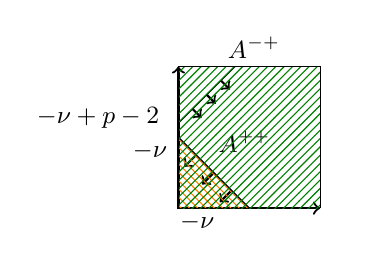
\begin{tikzpicture}[scale=0.6]
\draw [<->,thick] (0.0,3.0) node (yaxis) [above] {}
	|- (3.0,0.0) node (xaxis) [right] {};
\draw (0,1.5)  -- (1.5,0) ;
\draw [thick,->] (0.375,1.125) -- (0.125,0.875);
\draw [thick,->] (0.75,0.75) -- (0.5,0.5);
\draw [thick,->] (1.125,0.375) -- (0.875,0.125);
\node at (1.4,1.4) {\small $A^{++}$};
\node at (0.3999999999999999,-0.3) {\small $-\nu$};
\node at (-0.6,1.2) {\small $-\nu$};
\draw [pattern=north west lines, pattern color=orange] (1.5,0.0) -- (0.0,1.5) -- (0.0,0.0) ;
\draw (0.0,1.8) -- (1.2,3.0) ;
\draw [thick,->] (0.3,2.1) -- (0.49,1.9100000000000001);
\draw [thick,->] (0.6,2.4) -- (0.79,2.21);
\draw [thick,->] (0.8999999999999999,2.7) -- (1.0899999999999999,2.5100000000000002);
\node at (1.6,3.4) {\small $A^{-+}$};
\node at (-1.7,1.9000000000000001) {\small $-\nu+p-2$};
\draw [pattern=north east lines, pattern color=green!50!black] (3.0,0.0) -- (3.0,3.0) -- (0.0,3.0) -- (0.0,0.0) ;
\end{tikzpicture}}
\\[0pt]
			\toddText{\le n-3}&\input{f11}\\[0pt]
			\tevenText{>0}&\input{f12}\\[0pt]
			\toddText{>n-3}&\input{f13}\\[0pt]
		\end{tabular}
		\end{figure}
	\item $p\in\even,q\in\odd$とする。そうすると、$\nu\in\odd$ならば、 $R_{\lambda,\nu}^X$は射影函数である。そうではなかったら、(つまり、$\nu\in\even$ならば)、
	  \begin{figure}[H]
		  \noindent\begin{tabular}{@{}m{1.6cm}@{}ccc}
	      $(\lambda,\nu)\in$&$\mybra{//\cup\backslash\backslash}^c$ & $\backslash\backslash-//$  & $//\cap\backslash\backslash,k> l$\\[0pt]
	      \vspace{-3cm}$\nu\leq0$&\input{f14}\\[0pt]
	      \vspace{-3cm}$
	      \begin{array}{l}
		      \nu>0\\\nu\le\frac{n-3}{2}
	      \end{array}
	      $&\input{f15}\\[0pt]
              $(\lambda,\nu)\in$&$\mybra{//\cup\backslash\backslash}^c$ && $//\cap\backslash\backslash,k=l$\\[0pt]
	      \vspace{-3cm}$
	      \begin{array}{l}
		      \nu\todd\\\nu=\frac{n-1}{2}
	      \end{array}
	      $&\input{f16}\\[0pt]
	      $(\lambda,\nu)\in$&$\mybra{//\cup\backslash\backslash}^c$ & $//-\backslash\backslash$  & $//\cap\backslash\backslash,k< l$\\[0pt]
	      \vspace{-3cm}
	      $
	      \begin{array}{l}
		      \nu\ge\frac{n+1}{2}\\\nu\le n-3
	      \end{array}
	      $
	      &{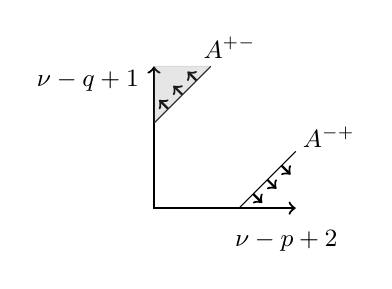
\begin{tikzpicture}[scale=0.6]
\draw [<->,thick] (0.0,3.0) node (yaxis) [above] {}
	|- (3.0,0.0) node (xaxis) [right] {};
\draw (1.8,0.0) -- (3.0,1.2) ;
\draw [thick,->] (2.1,0.3) -- (2.29,0.10999999999999999);
\draw [thick,->] (2.4,0.6) -- (2.59,0.41);
\draw [thick,->] (2.7,0.8999999999999999) -- (2.89,0.71);
\node at (3.7,1.5) {\small $A^{-+}$};
\node at (2.8,-0.7) {\small $\nu-p+2$};
\draw (0.0,1.8) -- (1.2,3.0) ;
\draw [thick,->] (0.3,2.1) -- (0.10999999999999999,2.29);
\draw [thick,->] (0.6,2.4) -- (0.41,2.59);
\draw [thick,->] (0.8999999999999999,2.7) -- (0.71,2.89);
\node at (1.6,3.4) {\small $A^{+-}$};
\node at (-1.4,2.7) {\small $\nu-q+1$};
\draw [fill=gray,opacity=0.2,gray] (0.0,1.8) -- (1.2,3.0) -- (0.0,3.0) ;
\end{tikzpicture}}
&{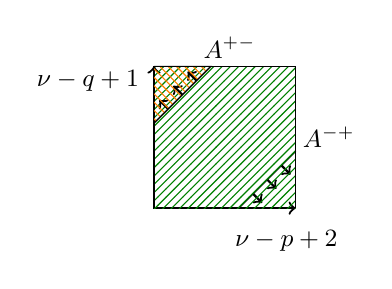
\begin{tikzpicture}[scale=0.6]
\draw [<->,thick] (0.0,3.0) node (yaxis) [above] {}
	|- (3.0,0.0) node (xaxis) [right] {};
\draw (1.8,0.0) -- (3.0,1.2) ;
\draw [thick,->] (2.1,0.3) -- (2.29,0.10999999999999999);
\draw [thick,->] (2.4,0.6) -- (2.59,0.41);
\draw [thick,->] (2.7,0.8999999999999999) -- (2.89,0.71);
\node at (3.7,1.5) {\small $A^{-+}$};
\node at (2.8,-0.7) {\small $\nu-p+2$};
\draw [pattern=north east lines, pattern color=green!50!black] (3.0,0.0) -- (3.0,3.0) -- (0.0,3.0) -- (0.0,0.0) ;
\draw (0.0,1.8) -- (1.2,3.0) ;
\draw [thick,->] (0.3,2.1) -- (0.10999999999999999,2.29);
\draw [thick,->] (0.6,2.4) -- (0.41,2.59);
\draw [thick,->] (0.8999999999999999,2.7) -- (0.71,2.89);
\node at (1.6,3.4) {\small $A^{+-}$};
\node at (-1.4,2.7) {\small $\nu-q+1$};
\draw [pattern=north west lines, pattern color=orange] (0.0,1.8) -- (1.2,3.0) -- (0.0,3.0) ;
\end{tikzpicture}}
&{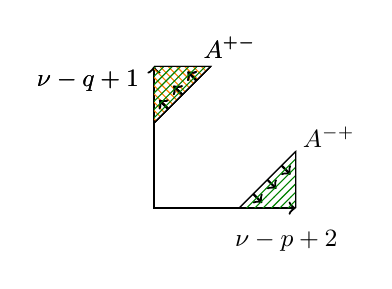
\begin{tikzpicture}[scale=0.6]
\draw [<->,thick] (0.0,3.0) node (yaxis) [above] {}
	|- (3.0,0.0) node (xaxis) [right] {};
\draw (1.8,0.0) -- (3.0,1.2) ;
\draw [thick,->] (2.1,0.3) -- (2.29,0.10999999999999999);
\draw [thick,->] (2.4,0.6) -- (2.59,0.41);
\draw [thick,->] (2.7,0.8999999999999999) -- (2.89,0.71);
\node at (3.7,1.5) {\small $A^{-+}$};
\node at (2.8,-0.7) {\small $\nu-p+2$};
\draw [pattern=north east lines, pattern color=green!50!black] (1.8,0.0) -- (3.0,1.2) -- (3.0,0.0) ;
\draw (0.0,1.8) -- (1.2,3.0) ;
\draw [thick,->] (0.3,2.1) -- (0.10999999999999999,2.29);
\draw [thick,->] (0.6,2.4) -- (0.41,2.59);
\draw [thick,->] (0.8999999999999999,2.7) -- (0.71,2.89);
\node at (1.6,3.4) {\small $A^{+-}$};
\node at (-1.4,2.7) {\small $\nu-q+1$};
\draw [pattern=north west lines, pattern color=orange] (0.0,1.8) -- (1.2,3.0) -- (0.0,3.0) ;
\draw (0.0,1.8) -- (1.2,3.0) ;
\draw [thick,->] (0.3,2.1) -- (0.10999999999999999,2.29);
\draw [thick,->] (0.6,2.4) -- (0.41,2.59);
\draw [thick,->] (0.8999999999999999,2.7) -- (0.71,2.89);
\node at (1.6,3.4) {\small $A^{+-}$};
\node at (-1.4,2.7) {\small $\nu-q+1$};
\draw [pattern=north east lines, pattern color=green!50!black] (0.0,1.8) -- (1.2,3.0) -- (0.0,3.0) ;
\end{tikzpicture}}
\\[0pt]
	      \vspace{-3cm}$
	      \nu>n-3$&\input{f18}\\[0pt]
	    \end{tabular}
	  \end{figure}
	\end{enumerate}
	\vspace{-0.9cm}
	In the diagrams above some of them are filled not with gray, but with colored diagonal lines. This means that the image of the regular
	SBO $R_{\lambda,\nu}^X$ is zero and the (green/purple)
	ascending/descending diagonal lines show the images of its residues $R_{\lambda,\nu}^{ \left\{ o \right\}}$ and $\tilde{R}_{\lambda,\nu}^X$ respectively.

	For $p=1$ we have:\\
	\newcommand{\mystack}[2]{$\begin{array}{l}#1\\#2\end{array}$}
	\begin{figure}[H]
		\begin{tabular}{p{3.2cm}p{2.0cm}p{2.0cm}p{2.0cm}p{2.3cm}p{2.3cm}}
		$(\lambda,\nu)\in$ & $\mybra{\ss\cup\bb}^c$ & $\ss-\bb$ & $\bb-\ss$ & $\ss\cap\bb,k<l$ & $\ss\cap\bb,k\geq l$\\
		\vspace{-0.7cm}\mystack{\nu\teven}{\nu\le0}&\input{f19}\\
		\vspace{-0.5cm}\mystack{\nu,q\teven}{0<\nu<q}&\input{f20}\\
		\vspace{-0.5cm}\mystack{\nu\teven,q\todd}{0<\nu<q}&\input{f21}\\
		\vspace{-0.7cm}\mystack{\nu,q\teven}{\nu\ge q}&\input{f22}\\
		\vspace{-0.7cm}\mystack{\nu\teven,q\todd}{\nu\ge q}&\input{f23}\\
		\vspace{-0.7cm}\mystack{\nu\todd,q\teven}{\nu\le0}&\input{f24}\\
		\vspace{-0.7cm}\mystack{\nu,q\todd}{\nu\le0}&\input{f25}\\
		\vspace{-0.5cm}\mystack{\nu\todd,q\teven}{0<\nu<q}&\input{f26}\\
		\vspace{-0.5cm}\mystack{\nu,q\todd}{0<\nu<q}&{
\begin{tikzpicture}[scale=0.6]
\draw[thick] (0.0,0.0)  -- (3.0,0.0) ;
\draw[fill=black] (0.0,0.0) circle (2pt);
\draw [fill=gray,opacity=0.2,gray] (-0.05,-0.36) -- (-0.05,0.36) -- (3.05,0.36) -- (3.05,-0.36) 
;\end{tikzpicture}}
&{
\begin{tikzpicture}[scale=0.6]
\draw[thick] (0.0,0.0)  -- (3.0,0.0) ;
\draw[fill=black] (0.0,0.0) circle (2pt);
\draw [fill=gray,opacity=0.2,gray] (-0.05,-0.36) -- (-0.05,0.36) -- (3.05,0.36) -- (3.05,-0.36) 
;\end{tikzpicture}}
&{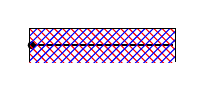
\begin{tikzpicture}[scale=0.6]
\draw[thick] (0.0,0.0)  -- (3.0,0.0) ;
\draw[fill=black] (0.0,0.0) circle (2pt);
\draw [pattern=north west lines, pattern color=red] (-0.05,-0.36) -- (-0.05,0.36) -- (3.05,0.36) -- (3.05,-0.36) 
;\draw [pattern=north east lines, pattern color=blue] (-0.05,-0.36) -- (-0.05,0.36) -- (3.05,0.36) -- (3.05,-0.36) 
;\end{tikzpicture}}
&{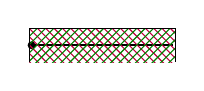
\begin{tikzpicture}[scale=0.6]
\draw[thick] (0.0,0.0)  -- (3.0,0.0) ;
\draw[fill=black] (0.0,0.0) circle (2pt);
\draw [pattern=north west lines, pattern color=purple] (-0.05,-0.36) -- (-0.05,0.36) -- (3.05,0.36) -- (3.05,-0.36) 
;\draw [pattern=north east lines, pattern color=green!50!black] (-0.05,-0.36) -- (-0.05,0.36) -- (3.05,0.36) -- (3.05,-0.36) 
;\end{tikzpicture}}
&{
\begin{tikzpicture}[scale=0.6]
\draw[thick] (0.0,0.0)  -- (3.0,0.0) ;
\draw[fill=black] (0.0,0.0) circle (2pt);
\draw [fill=gray,opacity=0.2,gray] (-0.05,-0.36) -- (-0.05,0.36) -- (3.05,0.36) -- (3.05,-0.36) 
;\end{tikzpicture}}
\\
		\vspace{-0.7cm}\mystack{\nu\todd,q\teven}{\nu\ge q}&{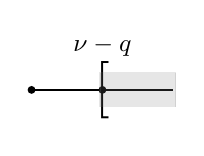
\begin{tikzpicture}[scale=0.6]
\draw[thick] (0.0,0.0)  -- (3.0,0.0) ;
\draw[fill=black] (0.0,0.0) circle (2pt);
\draw[fill=black] (1.5,0.0) circle (2pt);
\node at (1.5,0) {\huge [};
\node[align=center, above] at (1.5,0.5) {\small $\nu-q$}
;\draw [fill=gray,opacity=0.2,gray] (1.45,-0.36) -- (1.45,0.36) -- (3.05,0.36) -- (3.05,-0.36) 
;\end{tikzpicture}}
&{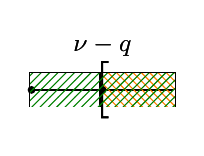
\begin{tikzpicture}[scale=0.6]
\draw[thick] (0.0,0.0)  -- (3.0,0.0) ;
\draw[fill=black] (0.0,0.0) circle (2pt);
\draw[fill=black] (1.5,0.0) circle (2pt);
\node at (1.5,0) {\huge [};
\node[align=center, above] at (1.5,0.5) {\small $\nu-q$}
;\draw [pattern=north west lines, pattern color=orange] (1.45,-0.36) -- (1.45,0.36) -- (3.05,0.36) -- (3.05,-0.36) 
;\draw[fill=black] (1.5,0.0) circle (2pt);
\node at (1.5,0) {\huge [};
\node[align=center, above] at (1.5,0.5) {\small $\nu-q$}
;\draw [pattern=north east lines, pattern color=green!50!black] (-0.05,-0.36) -- (-0.05,0.36) -- (3.05,0.36) -- (3.05,-0.36) 
;\end{tikzpicture}}
&{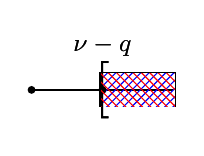
\begin{tikzpicture}[scale=0.6]
\draw[thick] (0.0,0.0)  -- (3.0,0.0) ;
\draw[fill=black] (0.0,0.0) circle (2pt);
\draw[fill=black] (1.5,0.0) circle (2pt);
\node at (1.5,0) {\huge [};
\node[align=center, above] at (1.5,0.5) {\small $\nu-q$}
;\draw [pattern=north east lines, pattern color=blue] (1.45,-0.36) -- (1.45,0.36) -- (3.05,0.36) -- (3.05,-0.36) 
;\draw[fill=black] (1.5,0.0) circle (2pt);
\node at (1.5,0) {\huge [};
\node[align=center, above] at (1.5,0.5) {\small $\nu-q$}
;\draw [pattern=north west lines, pattern color=red] (1.45,-0.36) -- (1.45,0.36) -- (3.05,0.36) -- (3.05,-0.36) 
;\end{tikzpicture}}
&{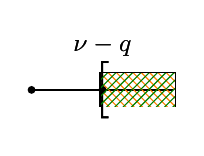
\begin{tikzpicture}[scale=0.6]
\draw[thick] (0.0,0.0)  -- (3.0,0.0) ;
\draw[fill=black] (0.0,0.0) circle (2pt);
\draw[fill=black] (1.5,0.0) circle (2pt);
\node at (1.5,0) {\huge [};
\node[align=center, above] at (1.5,0.5) {\small $\nu-q$}
;\draw [pattern=north west lines, pattern color=orange] (1.45,-0.36) -- (1.45,0.36) -- (3.05,0.36) -- (3.05,-0.36) 
;\draw[fill=black] (1.5,0.0) circle (2pt);
\node at (1.5,0) {\huge [};
\node[align=center, above] at (1.5,0.5) {\small $\nu-q$}
;\draw [pattern=north east lines, pattern color=green!50!black] (1.45,-0.36) -- (1.45,0.36) -- (3.05,0.36) -- (3.05,-0.36) 
;\end{tikzpicture}}
&{\vspace{-0.7cm}$\quad\;\;\quad\times$}
\\
		\vspace{-0.7cm}\mystack{\nu,q\todd}{\nu\ge q}&\input{f29}\\
	\end{tabular}\end{figure}
	In the diagrams above some of them are filled not with gray, but with colored diagonal lines. This means that the image of the regular SBO $R_{\lambda,\nu}^X$ is zero and:
	\begin{itemize}
		\item For $(\lambda,\nu)\in\ss$ the (green/purple)
			ascending/descending diagonal lines show the images of its residues $R_{\lambda,\nu}^{ \left\{ o \right\}}$ and $\tilde{R}_{\lambda,\nu}^X$ 
			respectively.
		\item For $(\lambda,\nu)\in\ss$ the (blue/red) ascending/descending diagonal lines show the images of its residues $R_{\lambda,\nu}^{Y}$ and ${R}_{\lambda,\nu}^C$ 
			respectively.
	\end{itemize}
\begin{remark}
	We can also find the images of the other SBOs in Theorem \ref{thm:construction} as well.
	Note that
	the proof of this theorem is performed \textit{independent of} of \cite{howe1993homogeneous}.
\end{remark}
Now, we recall from \cite{KO2} the five equivalent definitions of the
irreducible unitary representations $\pi_{\pm,\lambda}^{p,q}$ of $O(p,q)$.
\begin{theorem}[$G'$-invariant maps between Zuckerman modules $\pi_{\pm,\lambda}^{p,q}$]\label{thm:Aq}
	Let $n=p+q,\;(p,q\ge1)$ and $n':=n-1$.
	The dimensions of $\Hom_{G'}\left(\pi_{\pm,{n}/{2}-\lambda}^{p+1,q+1}\kern-0.3em\mid_{G'} ,\pi_{\pm,\nu-{n'}/{2}}^{p,q+1} \right)$
	are as follows:\newline
\ExecuteMetaData[.master_extract.tex]{Aq}\\\vspace{\baselineskip}
\begin{remark}
Theorem \ref{thm:Aq} generalizes \cite[Thms. 12.1 and 1.3]{kobayashi2015symmetry}.
\end{remark}
\end{theorem}
\nocite{kobayashi2015program}
\small
\bibliography{todai_master}
\bibliographystyle{mystyle}
\end{document}
